\documentclass{ltxdoc}
\usepackage{geometry}
\usepackage{phd}
\makeatletter
\newif\if@phdpreamble\@phdpreambletrue


\AtBeginDocument{\@phdpreamblefalse}
\makeatother
\usepackage{atbegshi}
\usepackage[pagelayout,savepos]{zref}
\sethyperref
%\luadirect{y='test'}

\makeatletter
\cxset{plain sections/.style={
 chapter name = CHAPTER,
 chapter toc = true,
 chapter color= thegray,
 chapter opening = right, 
 chapter numbering = arabic,
 chapter font-family= sffamily,
 chapter font-weight= bold,
 chapter font-size= LARGE,
 chapter before={\thinrule\vspace*{20pt}\par\hfill\hfill},
 chapter after={\vskip0pt\par},
 chapter spaceout = soul,
 number font-size= Large,
 number font-family= rmfamily,
 number font-weight= bfseries,
 number color=thegray,
 number before=\vspace*{5pt}\hfill\hfill,
 number dot=.,
 number after={\hspace*{7pt}\par},
 title beforeskip={\vspace*{10pt}},
 title afterskip={\vspace*{50pt}\par},
 title before={\hfill\hfill\raggedleft},
 title after={\par\thinrule},
 title font-family=\sffamily,
 title font-color= teal,
 title font-weight=\bfseries,
 title font-family=\sffamily,
 title font-size= Large,
 title font-shape= upshape,
 title spaceout= none,
 title beforeskip={\vspace*{10pt}},
 title afterskip={\vspace*{50pt}\par},
 title before={\hfill\hfill\raggedleft},
%
% numbers
% number font-family=\sffamily,
% number font-weight=\bfseries,
 number color=thelightgray,
 number before=\par\vspace*{5pt}\hfill\hfill,
 number dot=,
 number after={\hspace*{7pt}\par},
 number position=rightname,
 section color= thered,     
 section beforeskip=15pt,
 section afterskip=15pt,
 section indent=0pt,
 section font-family= sffamily,
 section font-size= LARGE,
 section font-weight= bfseries,
 section font-shape=,
 section align= centering,
 section numbering prefix =,%use \thechapter. for books or add as option
 section numbering= arabic,
 section spaceout=none,
 section number after=ooo,
 subsection color= thered,
       subsection beforeskip=10pt,
       subsection afterskip=10pt,
       subsection indent=0pt,
       subsection font-family= rmfamily,
       subsection font-size= large,
       subsection font-weight= bold,
       subsection font-shape= upshape,
       subsection align= centering,
       subsection numbering prefix=\thesection.,%\S\hairsp,%add . 
       subsection numbering custom =\@arabic\c@subsection,% \two@digits{\@arabic\c@subsection},%
       subsubsection color= gray,
       subsubsection beforeskip=5pt plus3pt minus 2pt,
       subsubsection afterskip=5pt,
       subsubsection indent=0pt,
       subsubsection font-family= rmfamily,
       subsubsection font-size= normalfont,
       subsubsection font-weight= bold,
       subsubsection font-shape= itshape,
       subsubsection align= centering,
       subsubsection numbering prefix =\thesubsection.\@arabic\c@subsubsection,
       subsubsection numbering custom =, %\two@digits{\@arabic\c@subsubsection},
       subsubsection number after =, 
%
       paragraph color= thegrey,
       paragraph beforeskip=,
       paragraph afterskip=-0.5em,
       paragraph indent=0pt,
       paragraph font-family= rmfamily,
       paragraph font-size= large,
       paragraph font-weight= bfseries,
       paragraph font-shape=,
       paragraph align= centering,
       paragraph number after = 0pt,
       paragraph numbering=numeric,
       subparagraph color= thered,
       subparagraph beforeskip=0pt,
       subparagraph afterskip=-.5em,
       subparagraph indent=0pt,
       subparagraph font-family= sffamily,
       subparagraph font-size= large,
       subparagraph font-weight= normalfont,
       subparagraph font-shape= slshape,
       subparagraph align= RaggedRight,
       subparagraph number after =, % can affect all needs checking
       %subsubsection numbering prefix=\S\hairsp\thesection,%add . here if need be
       subparagraph numbering=none,
}
}
\cxset{plain sections}
\cxset{style13/.style={
 name= {\protect\pan अमुकग्रन्थे},
 chapter spaceout = none,
 numbering=arabic,
 number font-size= HUGE,
 number font-family= sffamily,
 number font-weight= bfseries,
 number color= gray!50,
 number before=\par\vspace*{5pt}\hfill\hfill,
 number dot=,
 number after={\hspace*{7pt}\par},
 number position=rightname,
 chapter font-family= sffamily,
 chapter font-weight= bold,
 chapter font-size= LARGE,
 chapter before={\tikzrule\vspace*{20pt}\par\hfill\hfill},
 chapter color= black!50,
 title beforeskip={\vspace*{10pt}},
 title afterskip={\vspace*{50pt}\par},
 title before={\hfill\hfill\raggedleft},
 chapter rule color=teal,
 title after=\par\tikzrule,
 title font-family= sffamily,
 title font-color= teal,
 title font-weight= bfseries,
 title font-size= huge,
 section indent=-1em,
 section align= left,
 section numbering= arabic,
 section indent=0pt,
 section beforeskip=0pt,
 section afterskip= 10pt,
 section color=teal,
 subsection align= ,
 subsection font-family= sffamily,
 subsection font-weight= bfseries,
 subsection color = teal,
 subsection font-size= large,
 subsection font-shape=,
 subparagraph number after=,
 subsubsection align=,
}
}
\cxset{style13}

\renewparagraph
\renewsection
\renewsubsection
\renewsubparagraph
\renewsubsubsection

\makeatother
\AtBeginShipout{%
 \setbox\AtBeginShipoutBox=\vbox{%
  \vbox to 0pt{%
%\mbox{ \directlua{
%z=\thepage
%  tex.print('This is a test', z, y)
%}}
}
 \vbox to 0pt{{%
 \kern-1.5in %
 \hbox to 0pt{{%
 \kern-1.5in %
 \color{blue}%
 \rule{1in}{1in}%
 \hss
 }}%
 \vss
 }}%
 \hrule
 \hbox{\vrule\box\AtBeginShipoutBox\vrule}%
 \hrule
 }%
 }
\usepackage{makeidx}
 \makeindex
\begin{document}

testing \index{test}
\indexcommand[\textbar]{|}

\theindex
\printindex
\end{document}


\cxset{chapter name=chapter}
\cxset{chapter lua/.store in=\somecode}
\cxset{chapter lua=\luacode{ 
          y = 'some string' .. z}}
\mainmatter
\chapter{Test}
\section{test}

\makeatletter

\cxset{geometry textwidth/.store in=\textwidth@cx,
          geometry textheight/.store in=\textheight@cx,
          geometry tufte/.code={
             \newgeometry{a4paper,left=24.8mm,top=27.4mm,headsep=2\baselineskip,%
             textwidth=107mm,marginparsep=8.2mm,marginparwidth=49.4mm,%
             textheight=\textheight@cx\baselineskip,
             headheight=\baselineskip}
            \@twosidefalse \@mparswitchfalse 
    }
}


\def\pregeometry{\geometry{%
     left=74.8mm,
     top=27.4mm,
     headsep=2\baselineskip,%
     marginparsep=8.2mm,
     marginparwidth=49.4mm,
     textheight=\textheight@cx\baselineskip,%
     headheight=\baselineskip}%
     \@twosidefalse \@mparswitchfalse %
     \reversemarginpar}
\def\postgeometry{  \newgeometry{%
     left=74.8mm,
     top=27.4mm,
     headsep=2\baselineskip,%
     marginparsep=8.2mm,
     marginparwidth=49.4mm,
     textheight=\textheight@cx\baselineskip,%
     headheight=\baselineskip}%
     \@twosidefalse \@mparswitchfalse %
     \reversemarginpar}
\cxset{geometry oxford/.code=
\if@phdpreamble
    \expandafter\pregeometry
   \else
    \expandafter\postgeometry
   \fi
 }
   
  


\cxset{geometry textheight=49,
          geometry oxford,
           }
\cxset{marginpar push/.store in=\marginparpush@cx,
          marginpar font/.store in=\marginparfont@cx,
          marginpar justification/.is choice,
          marginpar justification/justifying/.code=\gdef\marginparjustification@cx{\justifying},
          marginpar justification/raggedright/.code=\gdef\marginparjustification@cx{\raggedright},
          marginpar justification/RaggedRight/.code=\gdef\marginparjustification@cx{\RaggedRight},
          marginpar justification/RaggedLeft/.code=\gdef\marginparjustification@cx{\RaggedLeft},
 }
\cxset{marginpar push=10pt,
          marginpar font=\normalfont\footnotesize\sffamily,
          marginpar justification=RaggedLeft}



%This is a sidenote without the footnote mark
\newcommand\marginnote[2][0pt]{%
  \marginpar{\hbox{}\vspace*{#1}\marginparfont@cx\marginparjustification@cx\vspace*{-1\baselineskip}\noindent #2}%
             
}


\def\asidecaption{\parbox{\marginparwidth}{{\bfseries Image \thefigure}\par\lorem}%
  \addtocontents{lof}{This is image 8}
}

\def\ps@caption{%
     \let\@oddfoot\@empty\let\@evenfoot\@empty%
     \edef\leftx{-\marginparwidth-\marginparsep}
    \def\@evenhead{%
           \begin{picture}(0,0)%
           \put(-\marginparwidth-\marginparsep,-\headheight-\topsep-5pt){ \line(1, 0){\marginparwidth}}%
           \put(-\marginparwidth-\marginparsep,-\headheight-\headsep){ \line(1, 0){\marginparwidth}}%
            \put(\leftx,-90){\asidecaption\par}%
            \stepcounter{figure}%
           \put(\leftx,-370){\asidecaption}%
        \end{picture}%
      }%
    \let\@oddhead\@evenhead%
    \let\@mkboth\@gobbletwo%
    \let\chaptermark\@gobble%
    \let\sectionmark\@gobble%
 }

\def\ps@bigpicture{%
    \setlength\headheight{19cm}%
    \let\@oddfoot\@empty\let\@evenfoot\@empty%
    \def\@evenhead{%
         \begin{picture}(0,0)%
          \put(-149,0){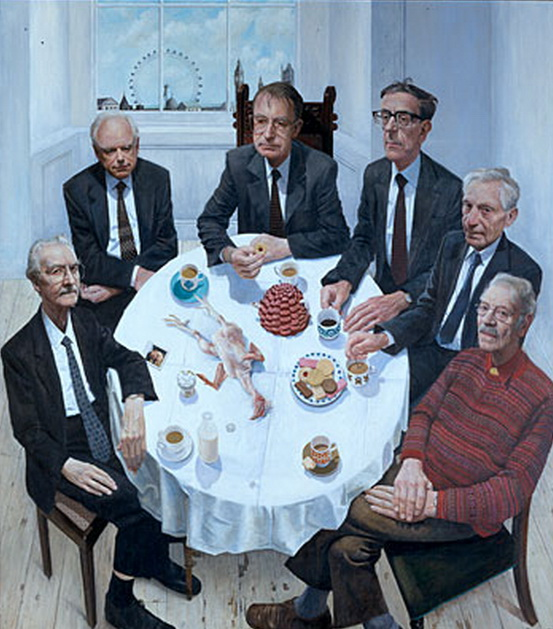
\includegraphics[width=\dimexpr(\textwidth+150pt)]{stuartpearson}}%
         \end{picture}%
      }%
    \let\@oddhead\@evenhead%
    \let\@mkboth\@gobbletwo%
    \let\chaptermark\@gobble%
    \let\sectionmark\@gobble%
 }


\def\doubletakeimage{%
  \renewcommand{\topfraction}{.95}%
  \begin{figure}[t]
      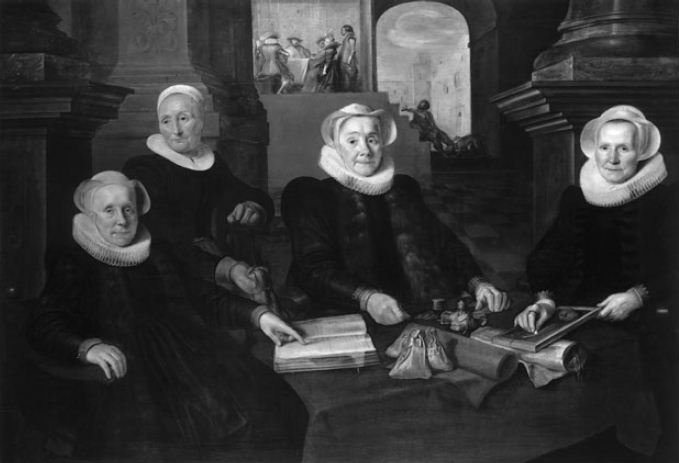
\includegraphics[width=\textwidth]{matron}%
       \thispagestyle{caption}
  \end{figure}

  \begin{figure}[tp]
   \hspace*{-\marginparwidth}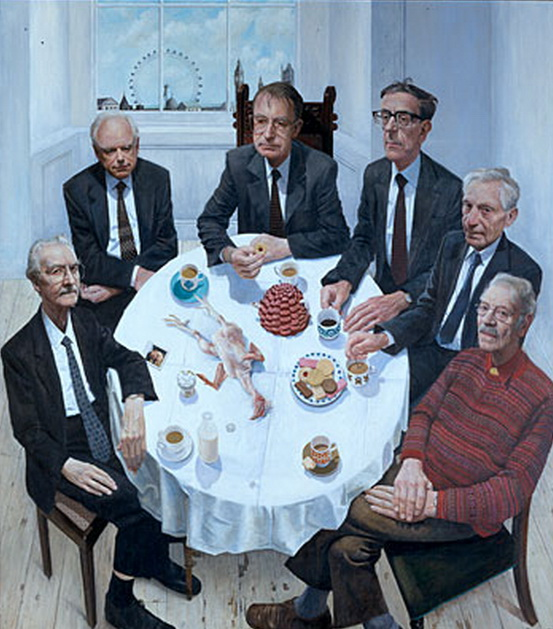
\includegraphics[height=0.9\textheight]{stuartpearson}
 \end{figure}
}



\chapter{Geometry and Page Dimensions}

Many modern books have pages with large margins, where either images or notes are added. The style we will
examine has mostly the captions of images. The advantage of such layouts is that firstly it improves the readability of the text by having shorter lines and secondly the images have reasonable dimensions. They also look very
good.

The textual treatment can easily be handled by \latexe so we will not be spending too much time discussing it, as 
we will focus our attention on the treatment of images and their captions.

The first thing we need to do is to specify the geometry of the page. Unlike Tufte’s books the Oxford University Press as well as the Cambridge University Press have all the margin material at the left. The \pkgname{phd} provides a style for such geometry named \textbf{oxford}

\begin{scriptexample}{}{}
\begin{verbatim}
\cxset{geometry=oxford}
\end{verbatim}
\end{scriptexample}

The interesting aspect of this style is the asynchronous floating of the margin captions as compared with
the images. 

\latexe’s   cs{marginpar} has not been designed with such problem in mind and is notoriously difficult
to get right especially if there are a lot of margninal material. The method I am proposing for here
is to use some of the abilities of pdfTeX engine to leverage the routines by using absolute positioning
thus in a way, we will build our own output routine rather than using the primitive cs{output} to process
the placement of the algorithm for images and their captions. 

Although the style is essentially what is termed a \texttt{oneside} style in real terms the captions (depending on the image size)  need to know if they are to be placed next to the image or at the previous page or at the next page margin. In practical terms the margin becomes another page. The typographical algorithm is described in the next section and the placement of the margin is a function of the image height and the set of page parameters $f: (i_h, p_m)$. 
For example if a page is a chapter opening page and is preceded  by a full page image then the caption is almost universally palaced at the bottom of the the chapter opening margin.

If we are to try and do all the manipulation ourselves rather than leaving it to standard \latexe routines, we will
need some helper macros and also we need to decide on the interaface we want to offer the user. 

\doubletakeimage

\section{Handling the image captions}

At first look the images should not present any difficulties and could be handled by normal
floating \latexe objects. On closer examination the larger images will need special treatment. In Fig~\ref{unequal}
the figure is shown as fullwidth, with the image caption placed in the margin of the \emph{previous} page. One of the major limitations of the \tex typesetting engine is that once a page is constructed the information on that page is lost. Before we attempt to program the palcements, let us define typographical rules for such image placements.

\begin{enumerate}
\item Measure the image width. If the image is $\le l_t$ then the image can be placed either at the top
         or bottom of the page and the side caption at the left of the image.
\item Measure the image height ($h_i$) and the height of the image caption ($h_{i,c}$). If the sum of the two exceeds the limit $l_m$ then signal that the image caption must be placed at the margin of the left page. If it does not then place it at the same page on top of the image.

\item Write the page object-1 to the auxiliary file.

\item When reading the auxiliary place the caption at the margin of the previous page. The placement will
depend on other marginal material, but preferably balance it by placing it at the bottom. 
\end{enumerate}
  
The central idea would be to write to the auxiliary file for every page, some information that we want to preserve
then we can by-pass to a large extend the output routine and tex engine limitations.

The information we need to be stored as an object of the form.

\begin{verbatim}
pagenumber = object(marginmaterial, placement preferences)
t = {pagenumber,
       image,
       caption,
       caption placement rules
       caption placement manual adjustments}
\end{verbatim}
 
\begin{figure}[tbp]
\fbox{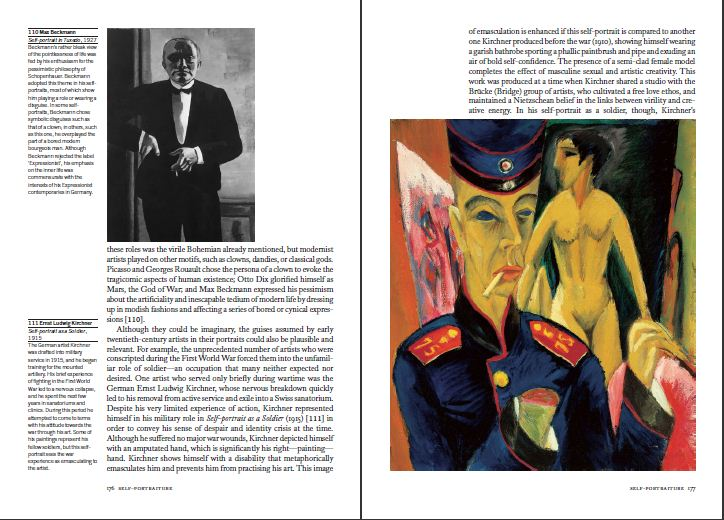
\includegraphics[width=\textwidth]{2-unequal-02}}
\caption{Page construction with the caption of the right page image, being placed on the margin of the page at the left. There is no standard way to automate such captions and images with \latexe, but with manual
intervention it is possible.}
\label{unequal}
\end{figure}

Another issue we need to handle is that images that are full width and height need to be treated differently. If they are on an even page then the caption needs to be moved forward to the next right page and placed either at the top or bottom, depending if the page has other images, if it is a heading opening page and the like.

The central idea to the algorithm is that all pages will have a page object defined and stored in the auxiliary
file. 

To achieve this we will try and define the objects using Lua rather than normal \tex routines although it could be as easy to do it with \tex commands. Writing to the auxiliary file should take place when we are in the output routine so that we can pick up the page number. This asynchronous or rather stateless output routine can be bypassed this way.\marginnote{See also similar routines that were developed as an extension to the Tufte-class.}

\begin{figure}[tbp]
\fbox{\includegraphics[width=\textwidth]{elizabeth}}
\caption{Page construction with the captioe  of the right page image, being placed on the margin of the page at the left. There is no standard way to automate such captions and images with \latexe, but with manual
intervention it is possible.}
\label{elizabeth}
\end{figure}

\begin{enumerate}
\item If full height image. If at the left page caption need to be placed at the right page.
\item If the right page has an image the caption of the left page needs to be placed first.
         For an example of this rule see Figure~\ref{elizabeth}.
\end{enumerate}

\section{Full width two images}

\begin{figure}[tbp]
\fbox{\includegraphics[width=\textwidth]{bazille}}
\caption{Page construction with the caption  of the right page image, being placed on the margin of the page at the left. There is no standard way to automate such captions and images with \latexe, but with manual
intervention it is possible.}
\label{elizabeth}
\end{figure}

Another interesting observation is what to do when we have to fullwidth images on the page. Again in ths case the image captions are placed on the next page. Here the captions are placed at preferred locations. The first caption
is set flush with the top margin and the second one is placed at the same height as the top of the image. What this means is that when the images are typeset we will  need to also store the position of the object at the page. This can also be observed on larger images see Figure~\ref{laura}

\begin{figure}[tbp]
\fbox{\includegraphics[width=\textwidth]{laura}}
\caption{Page construction with the captioe  of the right page image, being placed on the margin of the page at the left. There is no standard way to automate such captions and images with \latexe, but with manual
intervention it is possible.}
\label{elizabeth}
\makeatletter
%\write\@auxout{\protect\def\hello{hello \thepage}}


\end{figure}

\restoregeometry
A RESET EVERYTHING AT END OF CHAPTER


\addtocounter{chapter}{-2}
\@toctrue\@specialtrue


\lipsum[1-3]


 
\lipsum[1-50]








\end{document}